\chapter{Introducción}

Los objetos compactos (también llamados estrellas compactas) son el residuo de la vida luminosa de las estrellas y son llamados compactos porque su tamaño es significativamente más pequeño que el de una estrella en la secuencia principal con una masa similar. Como remanentes de estrellas, es pertinente revisar brevemente el proceso de formación y evolución estelar para tener una idea general de ... \TODO{Falta justificar en una línea por qué incluir el proceso de formación y evolución, y pulir.} 

Las estrellas son formadas a partir de nubes de gas interestelar, compuestas en su mayoría de hidrógeno molecular, que debido a algún tipo de perturbación (como una onda de choque) comienzan a colapsar sobre ellas mismas gravitacionalmente. La energía gravitacional es convertida en calor por la contracción y si la temperatura incrementa lo suficiente ($T \approx 10^7 \, \si{\kelvin}$, punto de ignición para la fusión de hidrógeno a helio), con ayuda de la contracción adicional causada por la pérdida de energía por radiación, la fusión se convierte en la fuente de energía principal y la presión termal y de radiación balancearán la gravedad, permitiendo así que la estrella se forme \cite{Glendenning2000CompactStars}.

Las reacciones nucleares pueden sostener la estrella por un gran periodo de tiempo (de millones a billones de años, dependiendo de la masa de la estrella) en lo que se conoce como su fase de secuencia principal, llamada así porque forman una secuencia mono-paramétrica (ignorando la composición química) cuyo parámetro es la masa estelar en el diagrama de Hertzsprung-Russell (Figura \ref{HR}) \cite{Scilla2016IntroductionEvolution}. 

\begin{figure}[H]
    \centering
    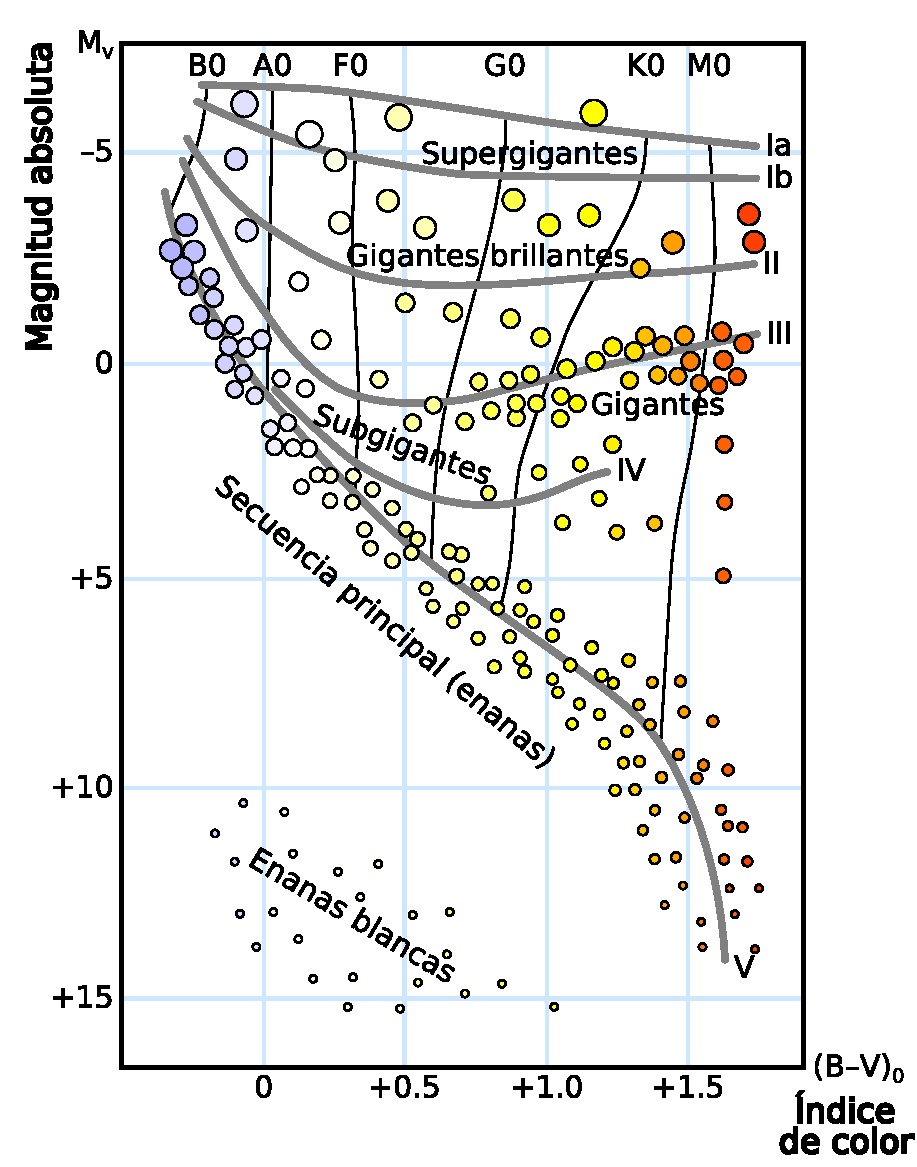
\includegraphics[width=200pt]{figures/H-R_diagram.pdf}
    \caption{Diagrama Hertzsprung-Russell}
    \label{HR}
\end{figure}

\begin{figure}[H]
    \centering
    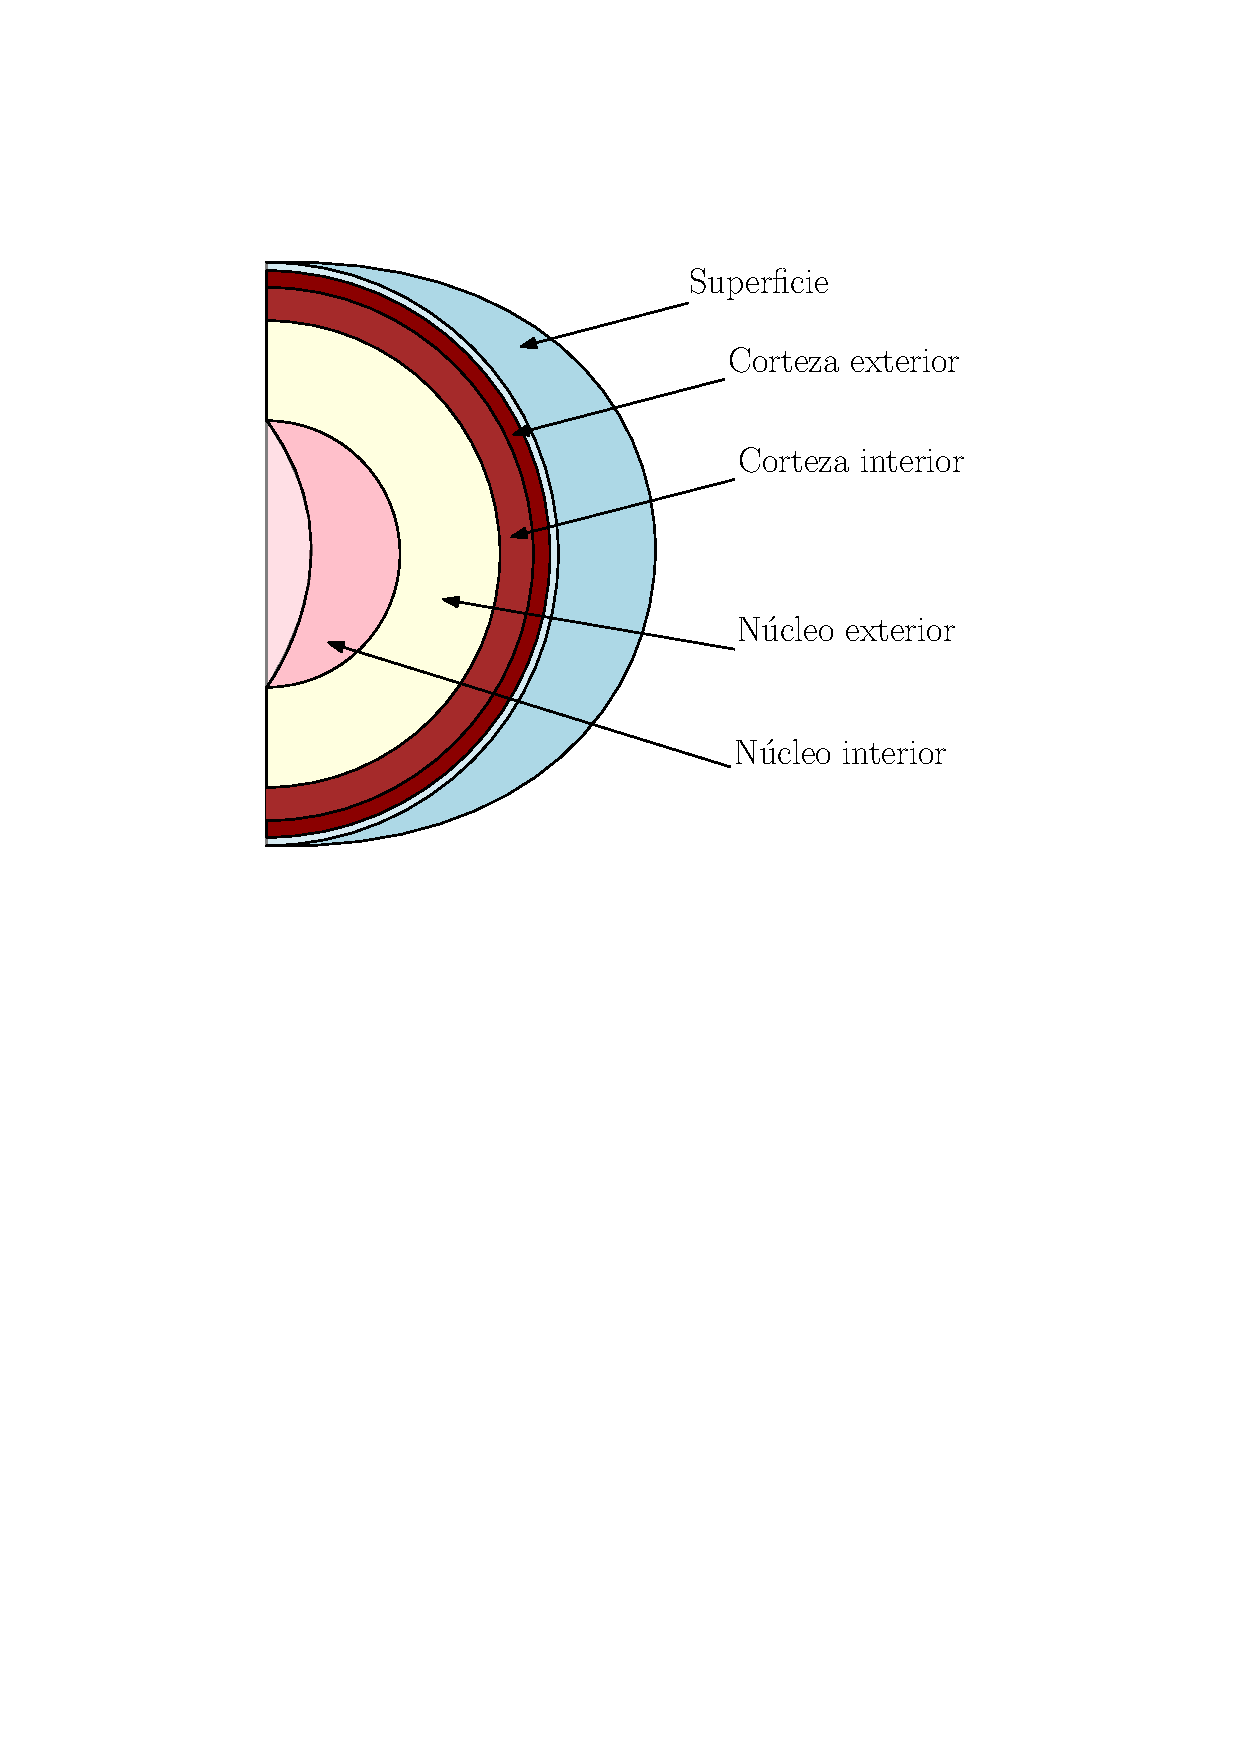
\includegraphics[width=200pt]{figures/neutronstar.pdf}
    \caption{Estructura interna de una estrella de neutrones}
    \label{NSS}
\end{figure}